\section{Implementation}
\label{sec:implementation}

While our proposed APIs are general and not language specific, we choose a safe
language, Rust, to implement our prototype. \sysname{} is open-source on
Github.\footnote{Url elided for anonymity.}  Applications built with \sysname{}
run as a single process.  The execution mode---profiling, runtime as client, or
runtime as server---is configurable with command line arguments or environment
variables.  Our deployment manager is currently a shell script.


\begin{table}
  \scriptsize
  \centering
  \begin{tabular}{c c c c}
    \toprule
    Application & Knobs & Accuracy & Dataset \\
    \midrule
    \specialcell{Augmented\\Reality}
                & \specialcell{resolution \\ frame rate \\ quantization }
                & F1 score~\cite{Rijsbergen:1979:IR:539927} & \specialcell{iPhone video clips\\training: office (24 s)\\testing: home
    (246 s)} \\
    \midrule
    \specialcell{Pedestrian\\Detection}
                & \specialcell{resolution \\ frame rate \\ quantization }
                & F1 score & \specialcell{MOT16~\cite{milan2016mot16}\\training: MOT16-04\\testing: MOT16-03} \\
    \midrule
    \specialcell{Log Analysis\\(Top-K)}
                & \specialcell{head (N) \\ threshold (T) }
                & \specialcell{Kendall's $\tau$~\cite{abdi2007kendall}}
                        & \specialcell{\href{https://www.sec.gov}{SEC.gov} logs~\cite{edgarlog} \\ training: 4 days \\
    testing: 16 days} \\
    \bottomrule
  \end{tabular}
  \caption{\sysname{} Applications}
  \label{tab:apps}
\end{table}


% First, Rust's memory safety guarantee can ensure applications running
% continously for an extended period of time. Besides, the zero-cost abstraction
% removes the possibilities of tail latencies caused by uncoordinated garbage
% collection~\cite{maas2016taurus}. In addition, we rely on Rust's type system
% to enforce the type match on \texttt{maybe} operations.

% All operators implement the \texttt{Stream} trait which has an associate type
% \texttt{Item} and a core function \texttt{next} that returns
% \texttt{Datum}. Each datum is either an item with the \texttt{Stream::Item} or
% an \texttt{Error} that the operator use to communicate with the runtime
% scheduler. The concrete form of \texttt{maybe} API is almost an direct
% translation of the API specification. While our API specification
% in~\autoref{tab:operators} uses a vector for knobs, our Rust implementation is
% more general: any type (including vector) that implements \texttt{IntoKnob}
% trait can be used as the knob.
% \begin{lstlisting}
% pub trait Stream {
%     type Item;
%     fn next(&mut self) -> Datum<Self::Item, Error>;

%     fn maybe<K, F>(self, opts: K, f: F) -> Maybe<Self, F>
%         where Self: Sized,
%                 K: IntoKnob,
%                 F: FnMut(K::Item, Self::Item) -> Self::Item {

%          // omitted
%     }
% }
% \end{lstlisting}

% \begin{figure*}
%   \centering
%   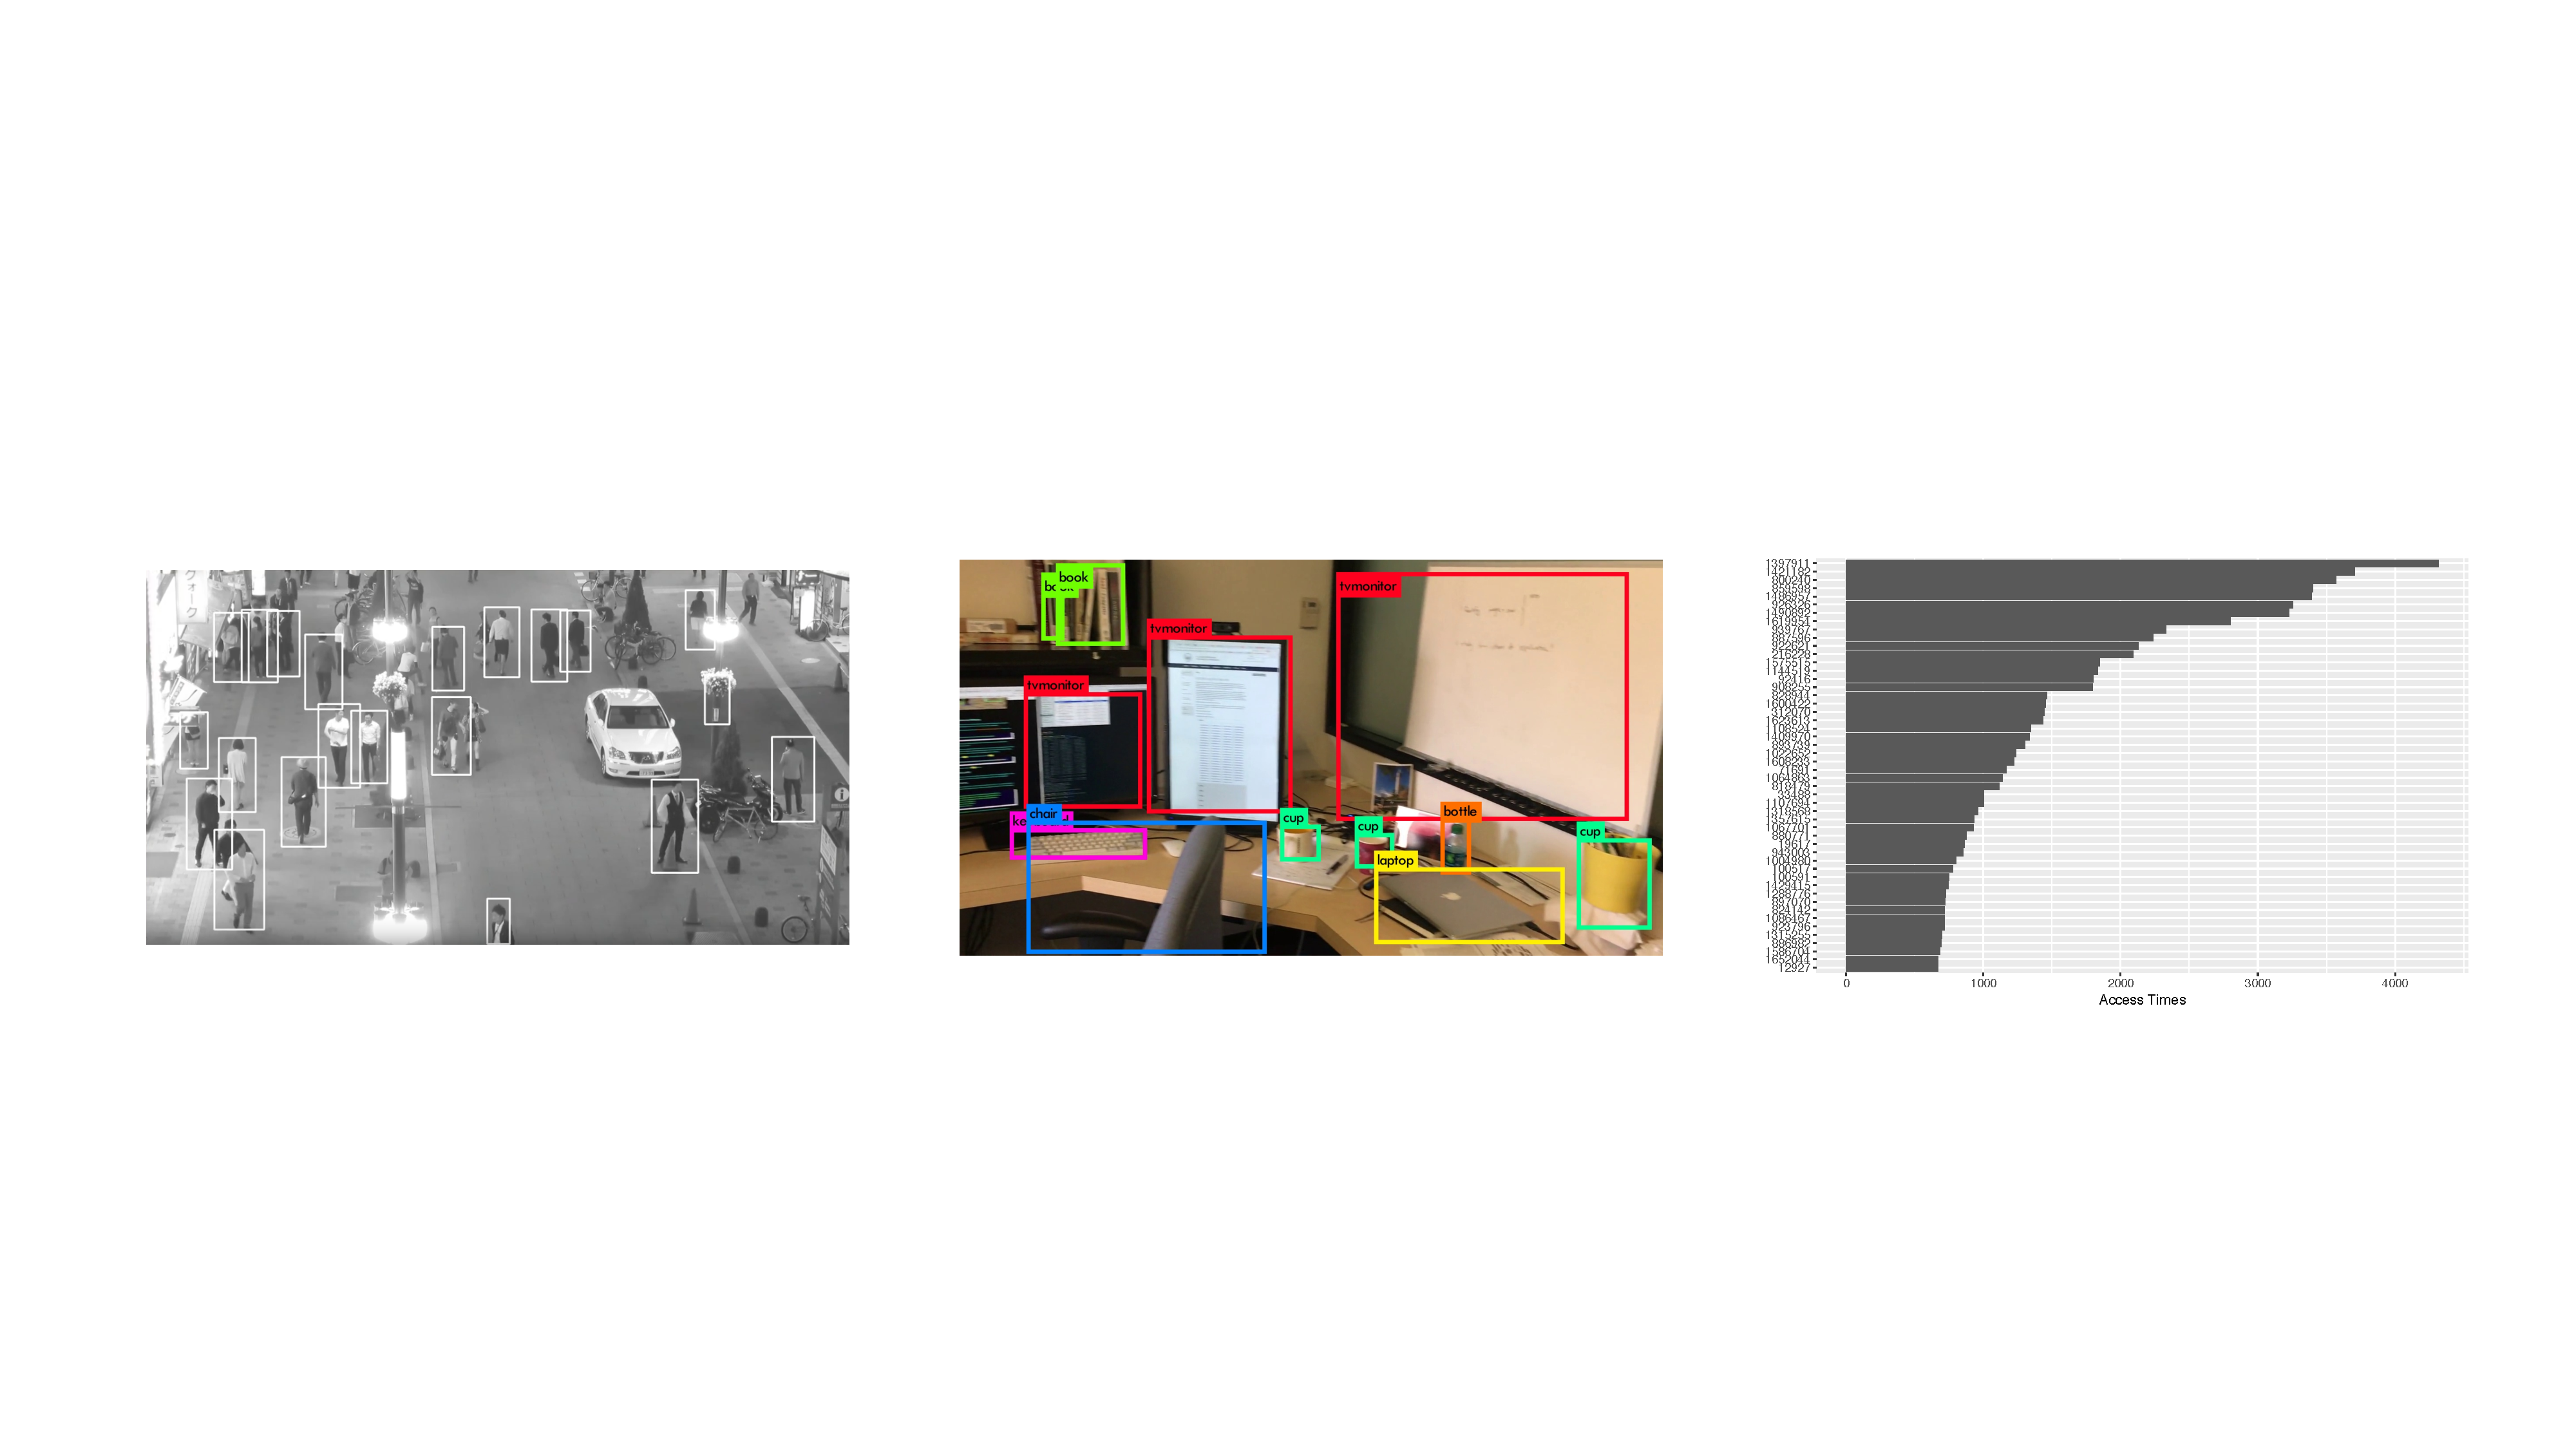
\includegraphics[width=\textwidth]{figures/apps.pdf}
%   \caption{Applications}
%   \label{fig:apps}
% \end{figure*}

We've built three applications: augmented reality, pedestrian detection, and a
distributed log analysis to extract the Top-K most access
files. \autoref{tab:apps} summarizes the application-specific part: knobs,
accuracy function, and the dataset we used for training and testing. The
implementation details of three applications are in the appendix.


%%% Local Variables:
%%% mode: latex
%%% TeX-master: "awstream"
%%% End:
